% Capítulo 5: rotação à direita (caso esquerda-esquerda da AVL).
\documentclass[border=4pt]{standalone}
\usepackage[utf8]{inputenc}
\usepackage[T1]{fontenc}
% Estilo comum das figuras de árvores (capítulo 5).
\usepackage{tikz}
\usetikzlibrary{arrows.meta, positioning, calc}
\definecolor{navy}{RGB}{23,45,80}
\definecolor{laranja}{RGB}{250,110,29}
\definecolor{cinzalogo}{RGB}{107,114,126}
\tikzset{
  vertice/.style={circle, draw=navy, line width=0.9pt, fill=laranja!12, minimum size=8mm,
                  inner sep=0pt, font=\sffamily\small},
  destaque/.style={vertice, fill=laranja!45, draw=laranja},
  apagado/.style={vertice, dashed, draw=cinzalogo, fill=white, text=cinzalogo},
  arvore/.style={level distance=12mm, edge from parent/.style={draw=navy, line width=0.9pt}},
  rotulo/.style={font=\sffamily\small\bfseries, text=navy},
  legenda/.style={font=\sffamily\scriptsize, text=cinzalogo},
  setanova/.style={-{Stealth[length=2.2mm]}, laranja, line width=1.3pt},
}

\tikzset{sub/.style={regular polygon, regular polygon sides=3, draw=cinzalogo, minimum size=9mm,
                     inner sep=0pt, font=\sffamily\scriptsize, text=cinzalogo}}
\usetikzlibrary{shapes.geometric}
\begin{document}
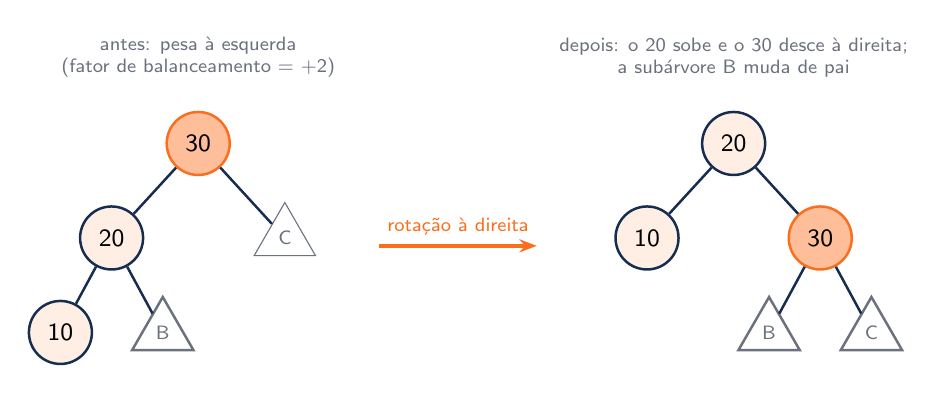
\begin{tikzpicture}[arvore, level 1/.style={sibling distance=22mm}, level 2/.style={sibling distance=13mm}]
  % antes
  \node[destaque] (y) at (0,0) {30}
    child {node[vertice] (x) {20}
      child {node[vertice] {10}}
      child {node[sub] {B}}}
    child {node[sub] {C}};
  \node[legenda, above=3mm of y, align=center] {antes: pesa à esquerda\\(fator de balanceamento = +2)};

  \draw[setanova] (2.3,-1.3) -- node[above, legenda, text=laranja] {rotação à direita} (4.3,-1.3);

  % depois
  \node[vertice] (x2) at (6.8,0) {20}
    child {node[vertice] {10}}
    child {node[destaque] {30}
      child {node[sub] {B}}
      child {node[sub] {C}}};
  \node[legenda, above=3mm of x2, align=center] {depois: o 20 sobe e o 30 desce à direita;\\a subárvore B muda de pai};
\end{tikzpicture}
\end{document}
